\documentclass{standalone}
\usepackage{tikz}
\usetikzlibrary{angles,quotes,math}

\begin{document}
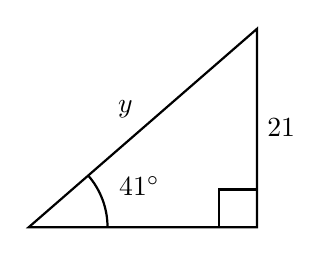
\begin{tikzpicture}[thick, scale=0.12]
  \coordinate (a) at (0,0);
  \coordinate (b) at (24.16,21);
  \coordinate (c) at (24.16,0);
  \draw
  (a) -- node[above left] {\(y\)}
  (b) pic["\(41^{\circ}\)", draw=black, -, angle eccentricity=1.5, angle radius=1cm]
  {angle=c--a--b} -- node[right] {\(21\)}
  (c) -- cycle;
  % Right angle square
  \draw (c) rectangle ++(-4,4);
\end{tikzpicture}
\end{document}
